% !TEX root = ../main.tex
%
\chapter{The (end of the) monocentric city}
\label{chap:monocentric_introduction}

\begin{flushright}{\slshape    
It may be a small irony that  
just as\\
the phenomenon of polycentricity\\ is getting considerable attention,\\
The world is moving beyond it.} \\ \medskip
--- Peter Gordon \& Harry Richardson~\cite{Gordon:1996}
\end{flushright}


\bigskip


The hypothesis that cities organise themselves around a single center of
activities -- often called Central Business District (CBD) in the U.S. -- may well
be one of the strongest hypotheses in urban studies. Although no one seriously
believes in its validity anymore, its influence is still creeping, often
unnoticed, in many empirical and theoretical works.  In order to deconstruct the
monocentric model, we first need to understand where it came from in the first
place, why it was introduced, and what evidence it was based on. 

In this chapter, we present a historical perspective on the monocentric
hypothesis. First, the context in which it was introduced, how it was gradually
realised that cities had a decentralised structure, and the emergence of the
notion of center. We then present a brief review of the methods and tools
developed to count their number. Finally, using American and Spanish data, we
show that larger cities are more polycentric. This suggests the existence of a
transition from a monocentric to a polycentric structure when the population of
cities increases.

\section{From monocentric, to polycentric cities}
\label{sec:introduction}

Maybe the least assuming way to represent the density profiles in cities is
through either cloropleth maps, or 3-dimensional representations. On cloropleth
maps, the $x$ and $y$ coordinates correspond to the original coordinates
projected on the plane. In the former case, the different values of density are
expressed by the use of different colors. This approach can be traced back as
far as $1898$ in Meuriot's \emph{Des agglom\'erations urbaines dans l'Europe
contemporaine}~\cite{Meuriot:1898} who drew a large number of density maps of
large Europen cities. He was later followed by Jefferson in
$1909$~\cite{Jefferson:1909} who did the same for several cities in the US,
Europe and Australia.\\


\begin{figure}
    \centering
    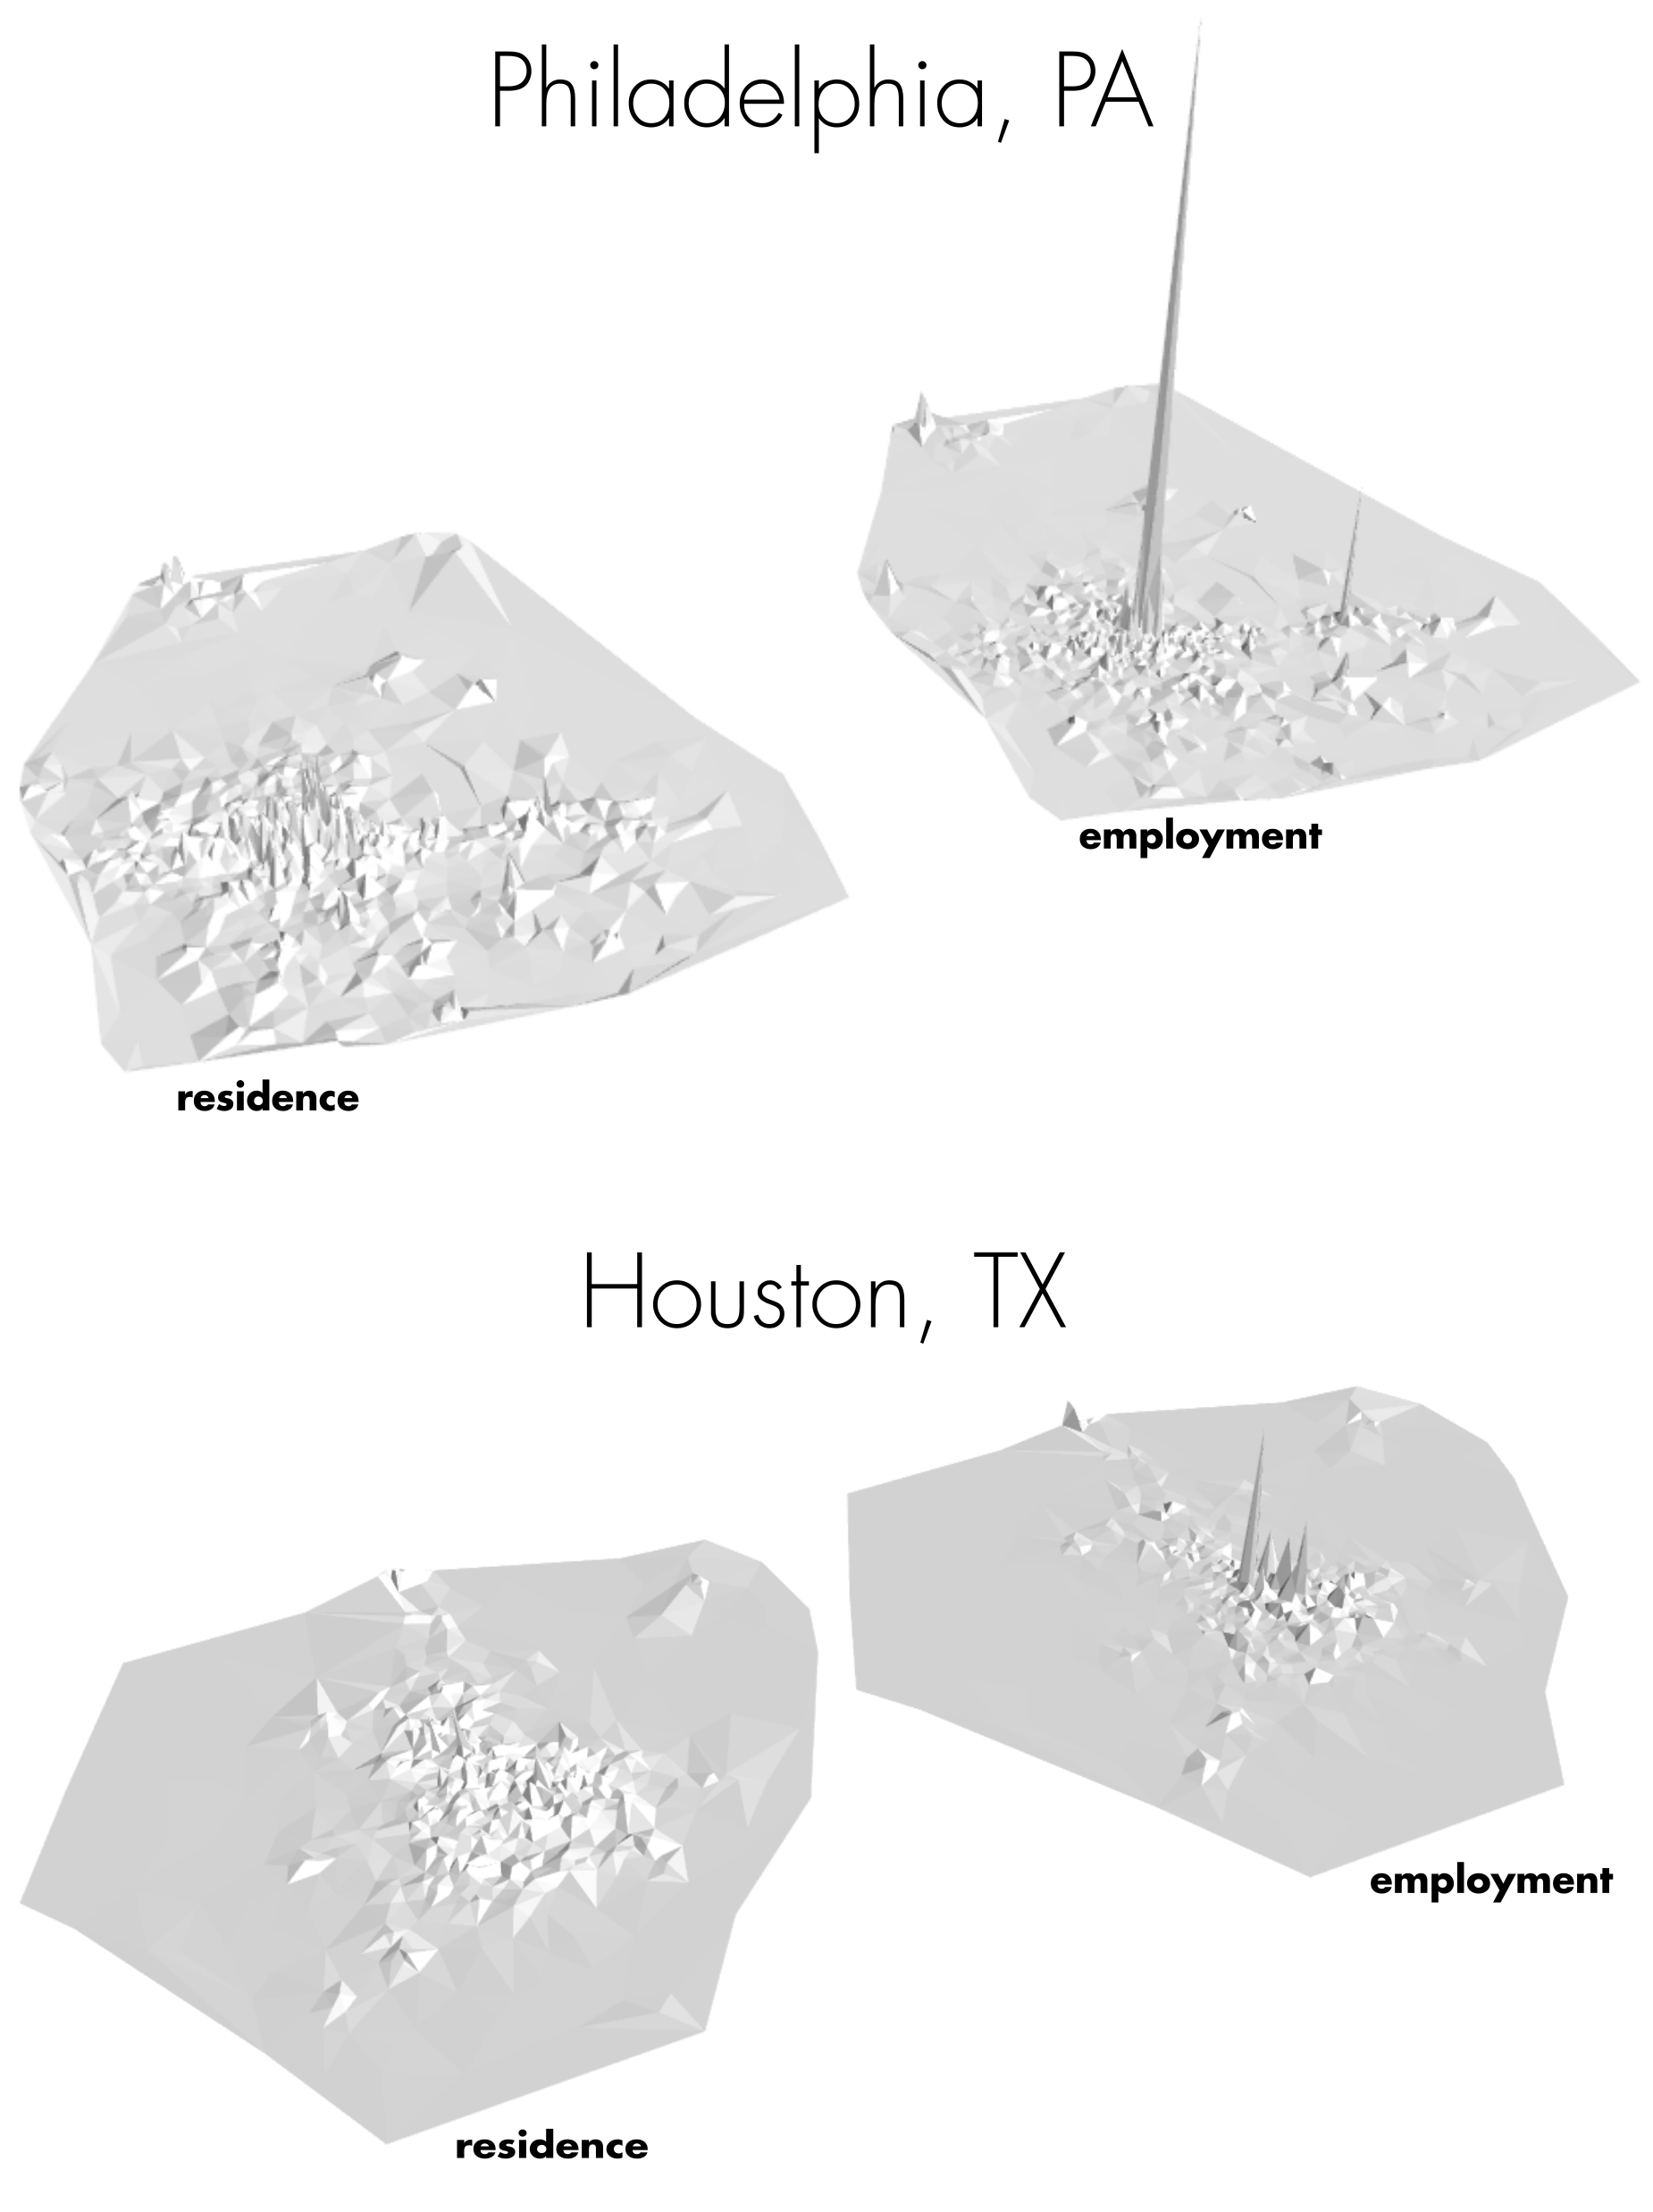
\includegraphics[width=\textwidth]{gfx/chapter-monocentric/panel_3d.png}
    \caption{{\bf 3D representations of densities.} Residential and
        employment densities in (Top) the Metropolitan Statistical Area (MSA) of
        Philadelphia, PA and (Bottom) the MSA of Houston, TX. Employment and
        residential densities are represented at the same scale.  Employment
        densities are sensibly more peaked than residential densities,
        suggesting that the notion of `center' is more relevant in the context of
        activies. Data were obtained from the 2000 US Census.  \label{fig:density_3d}}
\end{figure}


3-dimensional representations, on the other hand, use the $z$ coordinate to the
represent the density values. On Figure~\ref{fig:density_3d} we represent the
density profiles of two metropolitan areas in the US: Minneapolis-St.Paul, MN
and Houston, TX. These two cities are enough to illustrate the difficulties associated with
studying density profiles. 

\emph{What densities we are talking about?} People are constantly moving
throughout the city during the day, and density profiles can only be
(approximate) snapshots of the city at different instants.  Traditionally,
scholars have only considered residence densities (nightime city) and employment
densities (daytime city). The recent availability of mobile phone data may
however give us a more precise, continuous picture of the densities during the
day~\cite{Louail:2014}. In this part, we will be focusing on employment
densities.

\emph{How can we makes sense of these density patterns?} The densities represented
on Figure~\ref{fig:density_3d} are indeed very complex, and we would like to
isolate some particular structure. Arguably, the notion of center stems from
this desire to find some structure in the complex, messy empirical reality. \\

Realising that districts of large population tend to be central, and
districts of small population in the periphery, Clark proposes in
$1951$~\cite{Clark:1951} to write the density $\rho$ as a function of the
distance $d$ from the center

\begin{equation}
    \rho = a\,e^{-d/b} 
\end{equation}

Where $a$ is the density at the center, and $b$ the typical distance over which
the density decreases. To justify his assumption, Clark plots the population
density of various cities as a function of the distance to the
center~\cite{Clark:1951}. Some structure was found. The monocentric hypothesis
was born.\\


Looking at the density profiles plotted by Clark in 1951~\cite{Clark:1951} for
many cities across the world, or on Figure~\ref{fig:distance_center_minneapolis}
for the Minneapolis-St. Paul MSA, one can be
forgiven for thinking that cities have a monocentric structure. Such profiles
indeed almost always exhibit a sharp decrease as we go farther from the city
center -- defined here as the areal unit with the highest density. 

However, density profiles are not enough to prove the existence of a monocentric
structure. Unless one other hypothesis is verified: namely that the pattern of
employment densities is symmetric under rotations around the center. This is
however never the case: cities are nowhere isotropic but in the imagination of
modelers. To make this point clearer, we show on
Figure~\ref{fig:distance_center_minneapolis} both the density profile of the
Minneapolis-St. Paul MSA and a map where we highlight in black the tracts with
an employment density greater than $10000\,\text{km}^{-2}$. As one can see, two
tracts (respectively the historical centers of Minneapolis, and of St. Paul) are
highlighted. However, the peak in density corresponding to St. Paul is not
distinguishable on the density profile.  Indeed, it is averaged out with smaller
densities that are located at equidistance to Minneapolis. The decreasing
exponential model, however appealing, is thus mispecified.\\


\begin{figure}
    \centering
    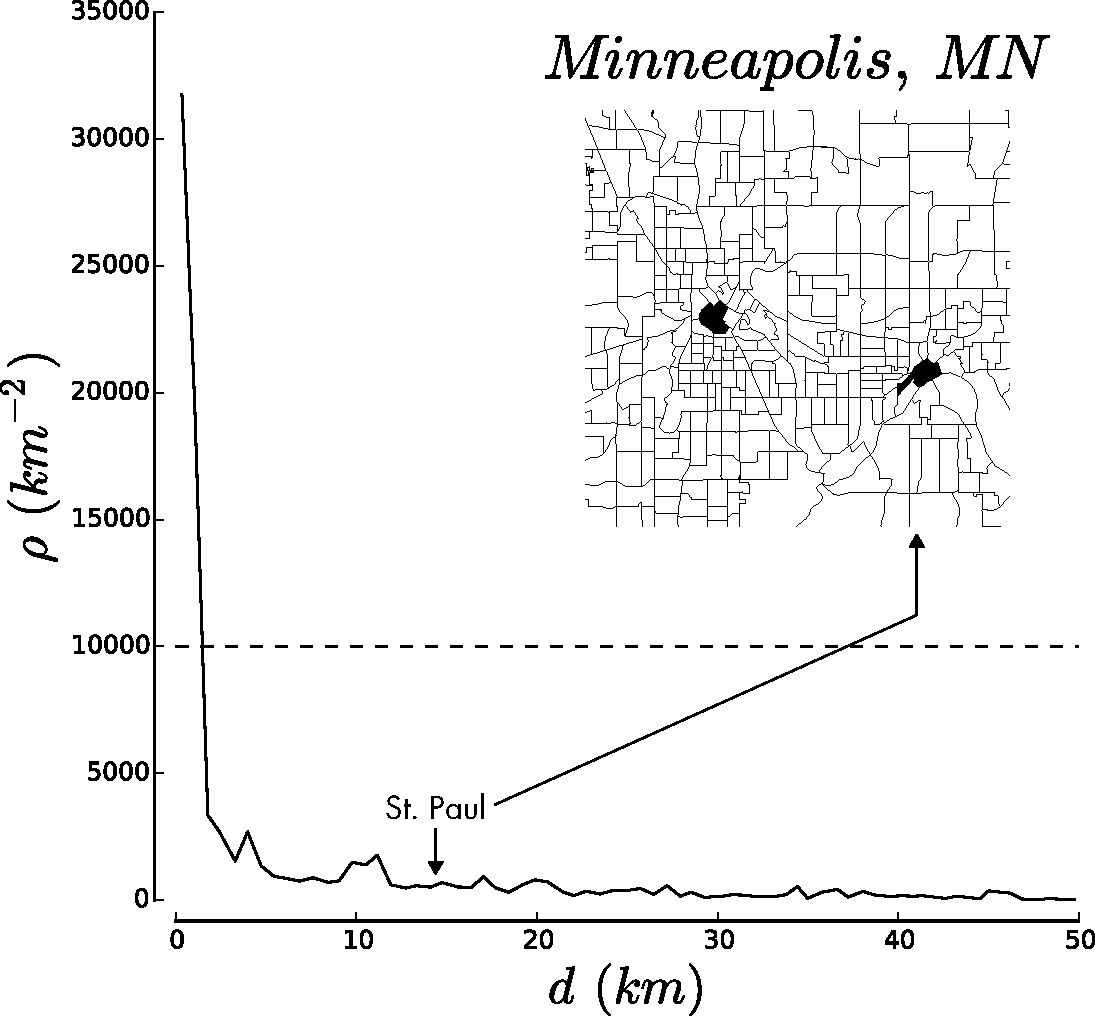
\includegraphics[width=\textwidth]{./gfx/chapter-monocentric/distance_center_minneapolis.pdf}
    \caption{{\bf The limitations of density profiles.} Employment density as a function of distance to the center for the
    Minneapolis-St. Paul MSA in $2000$. The center is defined here as the
    tract with the highest employment density, and corresponds to the historical
    Central Business District of Minneapolis. The curve exhibits a very sharp
    decay, giving the illusion of a monocentric structure. (Inset) The census tracts
    of Minneapolis-St. Paul in 2000. In black, the census tracts where the
    employment density reaches values above $10,000\,\text{km}^{-2}$. The two tracts
    coincide with the historical centers of the Twin Cities, and are distant from
    $14\,\text{km}$. This fragmented structure cannot be infered from the density
    profile (arrow on the curve).
    \label{fig:distance_center_minneapolis}}
\end{figure}


So why did Clark's methods and plots did not become a simple curiosity, but were
instead so widely adopted? Although it is sometimes difficult to trace back the
reasons for the adoption of ideas, there is little doubt that the echo this idea
had in urban economics had something to do with it (besides the simplicity of
the hypothesis). Indeed, beginning as an implied assumption in Clark's empirical
analyis, the monocentric hypothesis first became clearly stated in the
theoretical work of economists.


The Alonso-Muth-Mills model (inspired by Von Th\"unen's land rent model)  might
well be the reason for the long-lasting influence of the monocentric
model\footnote{A concise exposition of the AMM model can be found
in~\cite{Brueckner:1987,Fujita:1989}}. In 1964, Alonso introduced the bid-rent
curve as a function of the distance to the city center~\cite{Alonso:1964}. The
assumption that all firms in a city are concentrated in a single, fixed-size
part of the city naturally followed. Later, in $1967$ and $1969$,
Mills~\cite{Mills:1967} and Muth~\cite{Muth:1969} show how we can can obtain an
exponentially decreasing function for the density as a function of the distance
from the center, using the monocentric hypothesis. The monocentric
Alonso-Muth-Mills (AMM) model was born, and was seemingly backed by empirical
evidence.

One should not underestimate how the monocentric model influenced people's
perception of what a city is. In the US, the name of Central Business District
is casually used as a way to designate the principle activity center in a city.
Many, if not most, measures of the spatial variation of quantities inside cities
actually use the notion of `distance to the city center'. Many authors are
relying on the monocentric hypothesis for their empirical analysis -- sometimes
without being aware of it. This biais can still be found in the recent
literature. For instance, in a recent study by Glaeser, Kahn and Rappaport on the
repartition of income classes in cities~\cite{Glaeser:2008}, the authors comment
on plots of the average income as a function of the distance to the center. This
only makes sense, however, under the assumption of monocentricity.\\


This persistence of the monocentric hypothesis is all the more surprising that
authors repeatedly suggested and showed that the hypothesis was not adequate. In
$1974$, Kemper and Schmenner~\cite{Kemper:1974} explore industry and
employment density data, trying to fit a negative exponential function. Their
conclusion is clear: ``A declining exponential function fails to explain much of
the spatial variation of manufacturing density''. A few years later,
Odland~\cite{Odland:1978} explores the possibility of polycentric cities on a
theoretical basis. As explained in~\cite{Griffith:1981}, scholars subsequently started to
explore the density patterns of cities by fitting multi-center exponential
functions of the form

\begin{equation}
    \rho_i = \sum_{j=1}^{q} A_j\,e^{-d_{ij}/b_j}
    \label{eq:multi-exponential}
\end{equation}

where $\rho_i$ is the density at location $i$, $q$ the number of centers, $A_j$
the local maximum of density at $j$, $b_j$ the characteristic size of the center
$j$, and $d_{ij}$ the distance between locations $i$ and $j$. The idea of
polycentricity, originally as the generalisation of the monocentric hypothesis,
is progressively gaining ground. 

Trying to fit equations like Eq.~\ref{eq:multi-exponential} is cumbersome, and
requires some a-priori knowledge of the density patterns. It requires to
determine in advance which parts of the cities are going to be subcenters
\graffito{{\bf sub}center because they are subsidiary to the traditional CBD},
before attempting to fit the density profile. As noted in~\cite{Giuliano:1991},
authors used arbitrary definitions of subcenters, either designating them based
on their own intuition, or refering to the centers defined by planning agencies.
The centers were thus determined \emph{exogeneously}.\\

In this context, the first definitions of employment centers independent from
the exponential model start to emerge, and subcenters start an existence of
their own. By the $90$s, the idea that cities can be polycentric is
well-established, and more and more empirical analyses confirm the existence of
several employment centers. For instance, McDonald~\cite{McDonald:1987} identifies the
employment subcenters in the region of Chicago, IL; Giuliano and Small~\cite{Giuliano:1991} in the
region of Los Angeles, CA; Dokmeci et al.~\cite{Dokmeci:1994} show that Istanbul's employment
is spread across several centers, etc. 

The concept of subcenters is further expanded in $1991$~\cite{Garreau:1991},
when Garreau shows that secondary centers are not necessarily `subcenters'.
Indeed, activities do not always accumulate in the traditional downtown. He
introduces the concept of `Edge cities': the concentration of business, shopping
and entertainment at the outskirts of cities, in regions that were previously
rural, or purely residential.\\


\section{How to count centers}
\label{sec:how_to_measure_polycentrity}

The methods designed to identify employment subcenters can be divided in three
categories. The clustering methods, which appeared first, were progressively
abandonned for regression-based methods due to their reliance on arbitrary
cut-offs. Distribution-based methods have emerged recently, and leave
aside the spatial aspect of the density distribution.


\subsubsection{Clustering methods}
\label{ssub:clustering_methods}


In $1987$, McDonald~\cite{McDonald:1987} remarks that despite being mentionned
in the empirical and theoretical literature, the features that an employment
subcenter should have are nowhere discussed. For the first time, he proposes a method to
determine the number of subcenters empirically. Given
a number $T$ of areal units, we will say that $i$ with employment $E_i$,
population $P_i$ and surface area $A_i$ is an employment subcenter if:
\graffito{He also proposes a definition based on the employment-to-population
ratio}

\begin{quote}
    The gross employment density $\rho_i = E_i/A_i$ is greater than that of the
contiguous units; 
\end{quote}

Giuliano and Small~\cite{Giuliano:1991} acknowledge the necessity to
consider employment densities to define subcenters put forward by
McDonald~\cite{McDonald:1987}. However, they deplore that the method does not
allow for adjacent units with a high employment density to be centers -- as only
the larger one would be selected. Thus, they propose an alternate definition.
Namely that a contiguous set of units $\mathcal{S}$ is a subcenter if 

\begin{itemize}
    \item The employment density $\rho$ of every areal units in the set $\mathcal{S}$ is greater than
        a threshold value  $\overline{D}$;
    \item And the total employment $E$ contained in $\mathcal{S}$ is greater than a threshold
        $\overline{E}$.
\end{itemize}

where the thresholds $\overline{D}$ and $\overline{E}$ are imposed arbitrarily.
Using this definition, all areal units with a high employment densities are part
of a subcenter, unless they are small (contain less than $\overline{E}$
employees) or isolated (i.e. they do not belong to a cluster containing at
least $\overline{E}$ employees).\\


As mentioned by Anas et al. in~\cite{Anas:1998}, because density landscapes are highly
irregular at a small scale (see Figure~\ref{fig:density_3d} for instance), the
subcenter boundaries are very sensitive to the threshold values. Because there
is no a priori reason to choose a threshold rather than another, the obtained
subcenter boundaries are arbitrary and may vary from one author, one situation
to another. Instead, it would be preferable to have a method based on first
principles, that adapts to the local specificities.  In McMillen's words,
threshold methods lack a proper consideration of how large is `large' supposed
to mean for the threshold values~\cite{McMillen:2003}. 

Another problem highlighted in~\cite{Anas:1998} is that the number of centers
depends on the size of the areal unit, an issue that is tied to scale problem
discussed in the Modifiable Areal Unit Problem (MAUP)~\cite{Openshaw:1984}
literature. On the one hand, small areal units will lead to several low
employment density units in otherwise very high density areas. On the other
hand, large areal units are likely to smooth over local employment peaks. This
begs the question of whether we should use contiguity of units, or rather
distance, as a measure of proximity.


\subsubsection{Regression-based methods}
\label{ssub:regression_based_methods}

In an attempt to address these concerns, McMillen~\cite{McMillen:2001} proposes
a two stage procedure. In the first allegedly non-parametric stage, he uses a
geographically weighted regression (GRW, see~\cite{Brunsdon:1998} for more
details on the topic) to `smooth' the employment density, using distance rather
than contiguity as a measure of proximity, thus partially solving the issue
linked with the size of areal units.  The units that have unusually high
employment densities compared to the broad spatial trends obtained with the GWR are designated as
candidate subcenters. If we note $\rho_i$ the employment density at site $i$,
$\hat{\rho}_i$ the density estimated with GWR and $\hat{\sigma}_i$ the standard
deviation around this estimate, $i$ is said to be a \emph{candidate} subcenter
if 

\begin{equation*}
    \rho_i - \hat{\rho}_i > 1.96\,\hat{\sigma}_i
\end{equation*}

Candidate, because the GWR only identifies fluctuations in the density profile
with no consideration of whether these local fluctuations have a sensible impact
on the employment density. Identifying which of these candidates are actually
centers is the goal of the second, semi-parametric procedure. This second
procedure uses somewhat arbitrary criteria (the first and second largest
candidates are omitted in the regression, candidates at less than $1$ mile from
the CBD are omitted) to produce a second reference global trend, to which real values are
compared to identify the `real' centers among the candidates.\\

Redfearn critizes the first procedure~\cite{Redfearn:2007}, on the ground that candidate
subcenters are defined as outliers with respect to an average that uses half of the total
points (in the GWR), thus losing the local information about employment
density. The author proposes another non-parametric method that aims at correcting the issues
with McMillen's\cite{Redfearn:2007}. The estimation of the employment density is
done locally in order to keep intact the local structure of the density profile.
However, arbitrariness still lies in the choice of the span (the amount of data
that are considered to estimate the slopes at a given point) for the GRW. In
other words, regression-based methods are \emph{not} truly non-parametric.\\

\subsubsection{Distribution-based methods}
\label{ssub:distribution_based_methods}


The approach that we originally took in this thesis is radically different from
that of regression-based methods~\cite{Louf:2013_polycentric}. We start with the
remark that one does not need to know the spatial arrangement of areal units
with different densities in order to know which ones are most important. Indeed,
the local fluctuations that are registered as centers in the regression-based
methods are very likely to have a negligible contribution to the total
employment. They can thus be left out in a first approximation. A good estimate
of the number of centers should thus be given by the shape of the employment
density distribution alone. Because it does not require any spatial knowledge,
it makes the extraction of centers fairly easy and quick to compute compared to
the previous methods.\\

We start by building the rank plots of employment density $\rho$ inside the
areal units (see Figure~\ref{fig:rank_plot}). These plots display a decay at least as fast as that of an
exponential. If they were an exact exponential, they could be modeled by a
function of the form

\begin{equation}
    \rho(r) = \rho_0\,e^{-r/r_c}
    \label{eq:}
\end{equation}

\begin{figure}
    \centering
    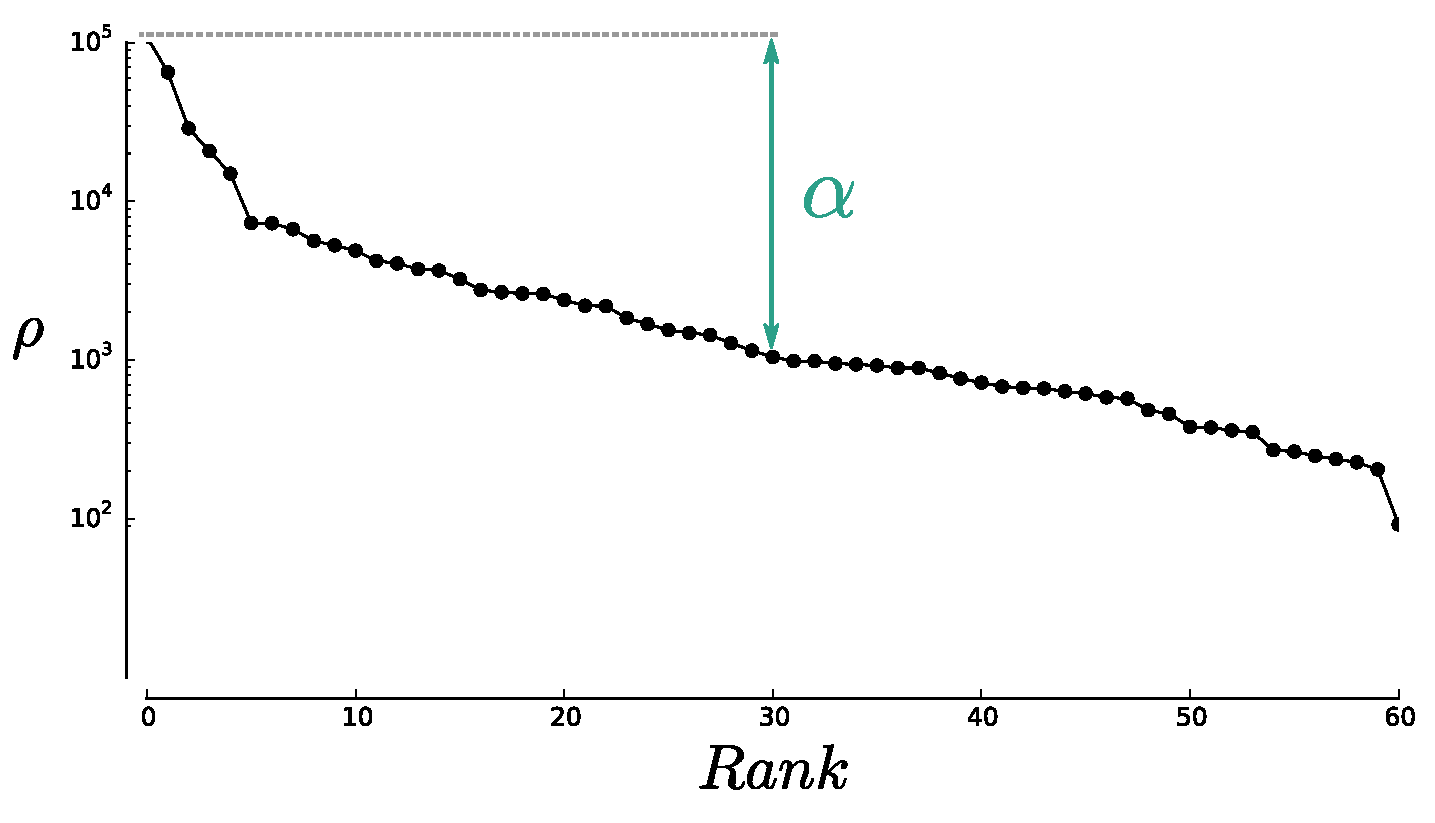
\includegraphics[width=1\textwidth]{gfx/chapter-monocentric/rank_plot_LA.pdf}
    \caption{{\bf The rank-plot method.} Rank plot of the employment density in
        the Zip Code Tabulation Areas of Los Angeles, CA.
    \label{fig:rank_plot}}
\end{figure}

where $\rho(r)$ is the $r$th highest value of the density inside the city,
$\rho_0$ the maximum density value. This exponential decrease implies that there
exists a natural scale for the rank, $r_c$, that we interpret here as the number
of centers. In order to get the number of centers, one would either need to
compute the slope on a lin-log plot, of find the value of $r^*$ for which

\begin{equation}
    \rho(r^*) = \frac{\rho_0}{e} 
\end{equation}

in which case $r^*=r_c$. However, empirical rank plots are not strictly exponential,
and we define the number of centers using a threshold value $\alpha$. We define
$\rho_m$ as 

\begin{equation}
    \rho_m = \frac{\rho_0}{\alpha}
\end{equation}

and the number of subcenters $k$ is equal to the number of values $\rho_c$ of
the density such that $\rho_c \in \left[ \rho_m, \rho_0 \right]$. 

In the case where the rank plot would be strictly exponential, we would have

\begin{equation}
    k = \rho_0\,\ln \alpha
\end{equation}

so that the number of centers is mainly determined by $\rho_0$. Small variations
in $\alpha$ should not sensibly change the number $k$ of centers obtained.

The method however suffers from two flaws. First, the use of an arbitrary
parameter, the threshold $\alpha$ to extract the number of centers. All the criticisms listed earlier also apply: we are not sure to extract the
`true' number of centers. Moreover, the method assumes a particular form for
the density distribution, which is likely to biais the estimation.\\

Louail and Barthelemy~\cite{Louail:2014} propose a generalisation of the
previous method based on the Lorenz curve. \graffito{The Lorentz curve is often
used in Economics to quantify income inequality.} Given the ordered set of
densities $\rho_1 < \rho_2 < \dots < \rho_T$ in the $T$ units, we plot the
proportion of cells $F_i=i/T$ as a function of the corresponding proportion of
employment density

\begin{equation}
    L_i = \frac{\sum_{n=1}^i \rho_n}{\sum_{n=1}^T \rho_n}
\end{equation}

so that both $F_i$ and $L_i$ take their values between $0$ and $1$ (see 
Figure~\ref{fig:loubar}). It is easy
to see that, in the case of a city with a uniform employment density, the
Lorentz curve is a straight line. In the general case, however, the curve has a
convex shape, with a more or less pronounced curvature.  The higher the
curvature of the Lorentz curve, the higher the inequality in terms of employment
density, and thus the smaller the number of potential centers. 

Following this observation, the authors define a new criterion to determine the number of
centers. They consider the intersection $F^*$ between the tangent of the
Lorentz curve at the point $L(F) = 1$ and the axis $F=0$ (see
Figure~\ref{fig:loubar}. The units that correspond to the values of $F$ between
$F^*$ and $1$ are defined as centers. This definition has the merit to only
depend on the distribution of density inside the areal units; it is \emph{genuinely
non-parametric}, while being easily tractable and understandable.\\

\begin{figure}
    \centering
    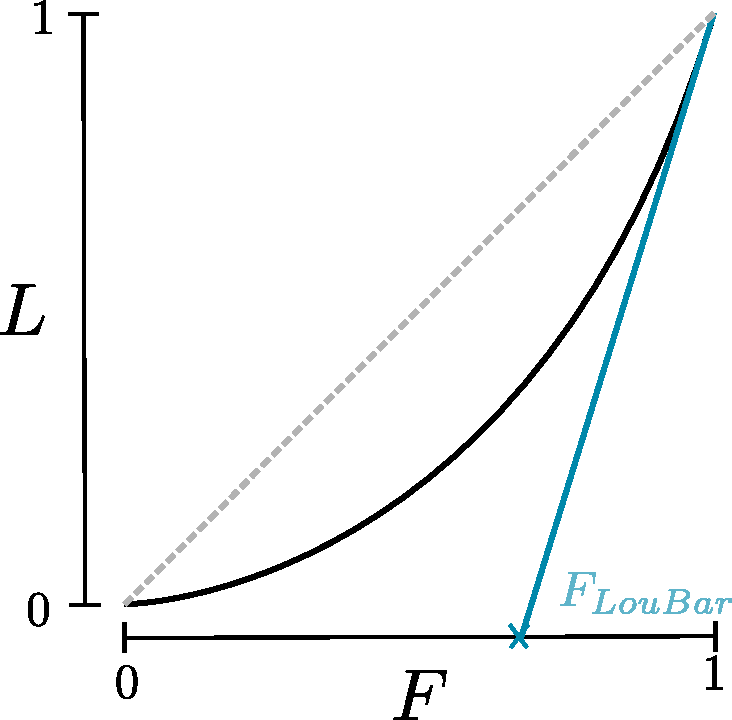
\includegraphics[width=0.6\textwidth]{gfx/chapter-monocentric/loubar.pdf}
    \caption{{\bf Lorentz curve and Loubar method.} An example of realistic Lorentz curve (solid black line), the curve
    that would be obtained in a city with uniformly distributed density (dashed
    grey line), and the tangent at the point $L(F) = 1$ (blue line) used to determine the number
of centers in the LouBar method.\label{fig:loubar}}
\end{figure}

Of course, all the methods presented here have issues (that we discuss 
in Chapter~\ref{chap:monocentric_discussion}), and there is currently no
consensus on what method should be used to find the employment centers.
More work is needed before we arrive at a satisfactory description of
urban form. Nevertheless, the results given by these methods -- although slightly
different -- provide together a compelling evidence for the polycentric
structure of cities. 


\section{The polycentric transition}
\label{sec:the_polycentric_transition}

Occasionnally mentioned in the empirical literature~\cite{McMillen:2003,
Redfearn:2007}, and hinted at in urban economics models~\cite{Fujita:1982},
the greater polycentricity of larger cities was not firmly established before
this thesis. Almost all cities (apart from the notable exception of twin cities)
start growing around a single center of activity. Yet, as we will see, no large
city adopts a strict monocentric structure. Therefore, it seems that, as
they grow and expand, urban systems develop a more and more polycentric form. We
call this phenomenon the `polycentric transition' of cities. 

\subsection{Empirical evidence}
\label{sub:empirical_evidence}

\subsubsection{American cities (Census data)}
\label{ssub:american_cities_census_data_}

Historical data over long periods of time, on a consistent set of areal units,
are very rare -- if not impossible to find. However, we do, for one point in
time, have many cities with very different population values. We can thus compute
and plot the number of centers as a function of population. Of course, as we
will discuss in more details in Part~\ref{part:scaling}, there is a gap between
time series and transversal studies that is not completely obvious to
bridge. Some cities can be, for historical reasons, locked into a monocentric
state when the average city would not. For different reasons, another city
might as well have developped a polycentric structure more prounounced than
other cities of the same size have. The idea here is to look at a large number
of cities and measure the average behaviour of this ensemble of cities, hoping
that marginal cases are indeed marginal.

% Corrections until here

\subsubsection{American cities (census data)}
\label{ssub:american_cities_census_data_}

During this thesis~\cite{Louf:2013_polycentric}, we used data on the employment in the Zip Codes of US cities
every year between 1994 and 2010. We first extracted the number of
centers for every city, for every year between 1994 and 2010. Using the
rank-plot method described earlier. We then applied the following treatment to
the data:

\begin{itemize}
    \item If there is only one Zip Code in the given city, $k=1$;
    \item We perform a Kolmogorov-Smirnov test~\cite{Massey:1951} between the
        distributions of a given city for consecutive years. If there is a
        significant difference (above a threshold $p_{KS}$) between the
        distribution at $t$ and $t+1$, we keep the point at $t+1$. If there is
        no sensible difference, we discard it.
\end{itemize}

At the end of this process, we obtain points that can be understood as coming
from different realisations of a city. We then plot the number of centers
computed for all these realisations as a function of the total population and
obtain the curve obtained on Figure~\ref{fig:us_centers}.

\begin{figure}
    \centering
    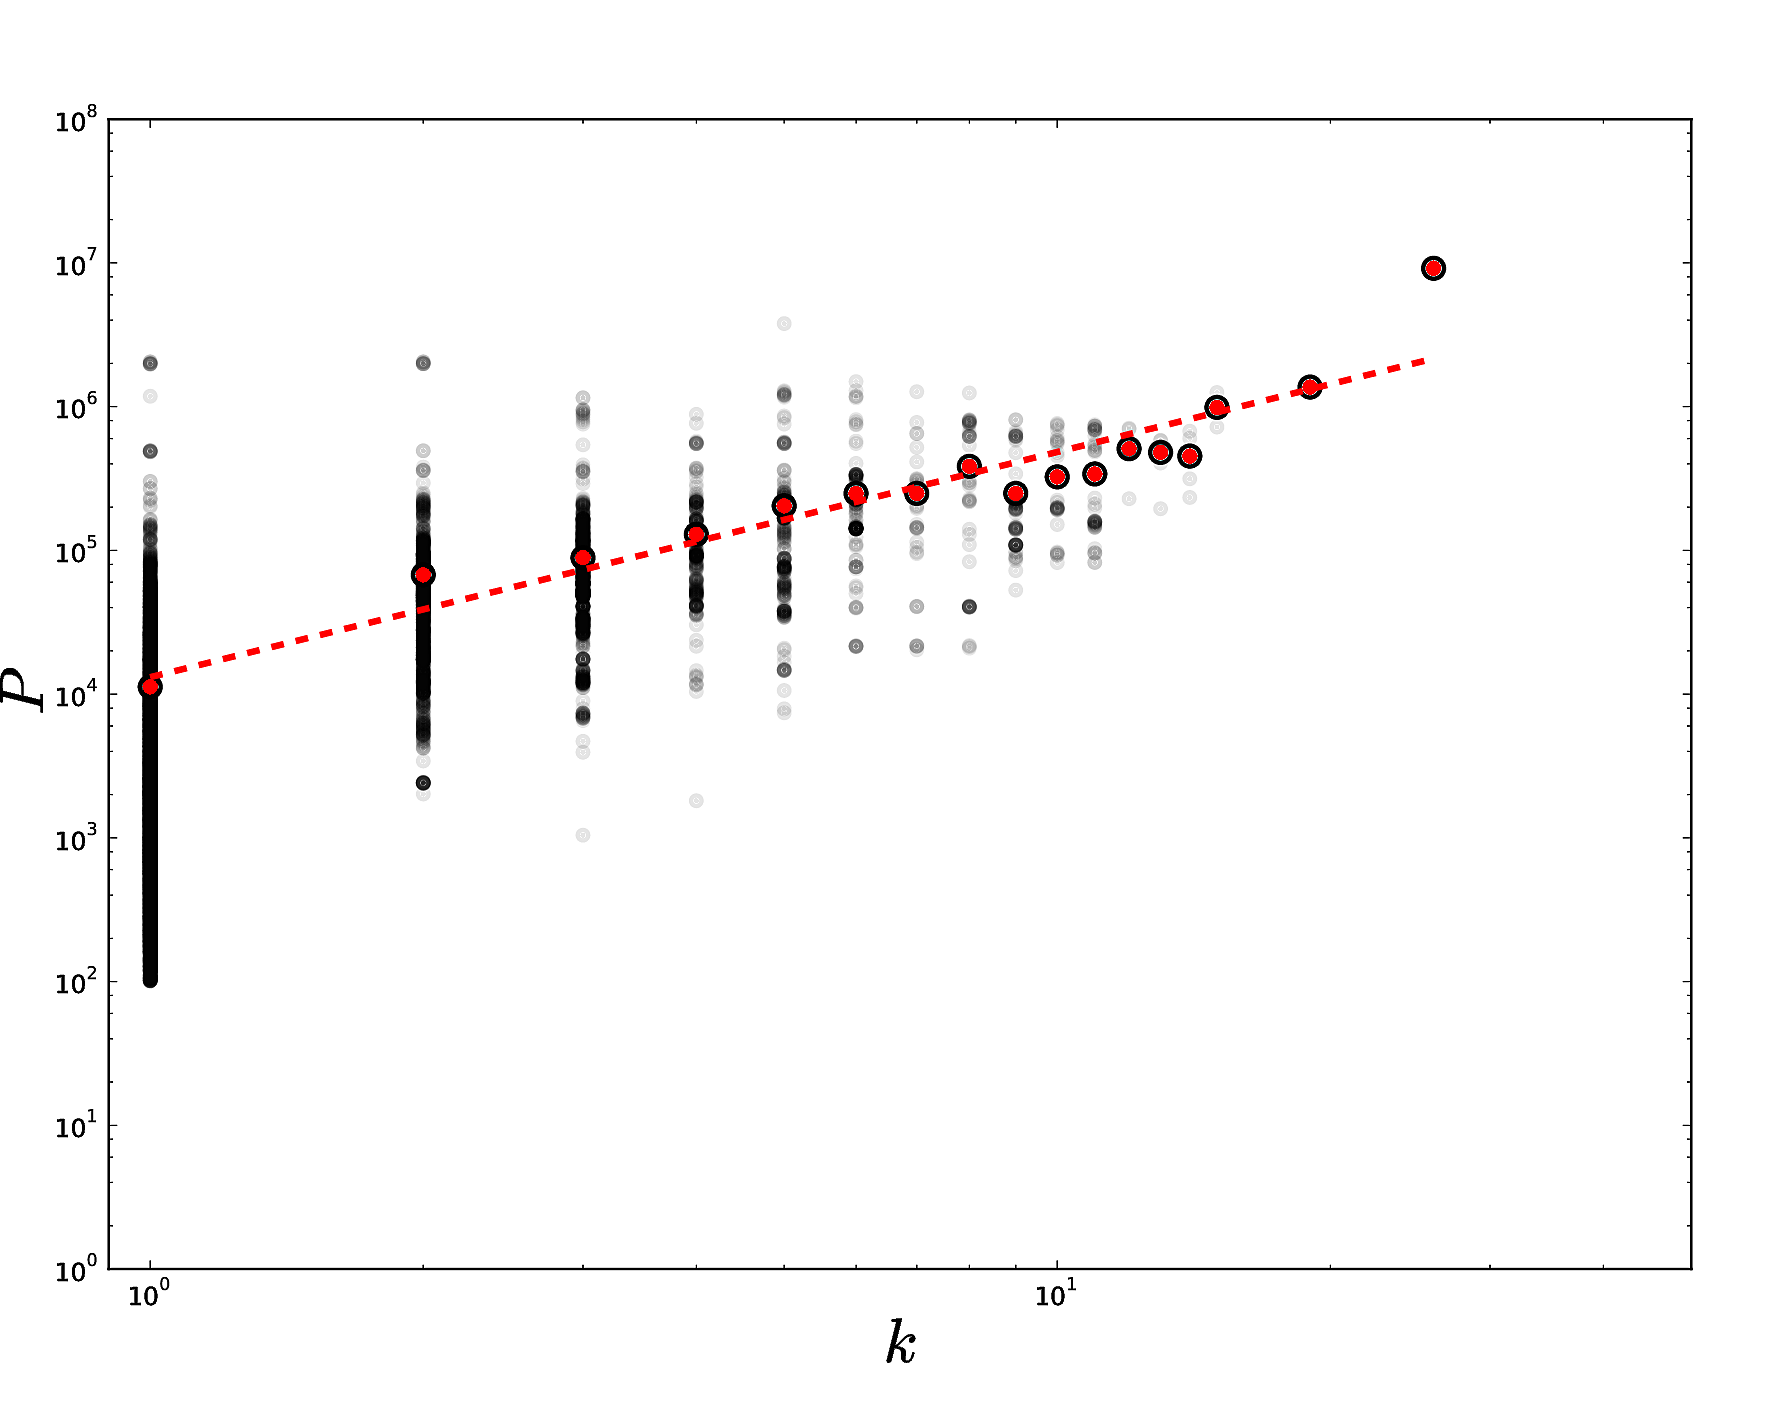
\includegraphics[width=0.9\textwidth]{gfx/chapter-monocentric/5.png}
    \caption{{\bf Centers in American cities.} Scatter plot for the estimated number of centers versus the
    population for about 9000 cities (different realisations) in the US. The red
dots represent the average population for a given number of subcenters. We fit
this average assuming a power-law dependence giving an exponent $\delta = 1.56
    \pm 0.15\,(R^2=0.87)$. Data were obtained from the U.S. Census Bureau's Zip
Code Business Patterns for every year between $1994$ and $2010$. \label{fig:us_centers}}
\end{figure}


A power-law fit on the average per population bin gives an exponent $\delta =
1.56 \pm 0.15\,(95\%\,C.I.)$. Thus, we find that on average, the number of
centers in U.S. cities scales with population size as

\begin{equation}
    k_{\,US} \sim P^{\,0.64}
\end{equation}

\subsubsection{Spanish cities (mobile phone data)}
\label{sub:spanish_cities_mobile_phone_data_}

\begin{figure}
    \centering
    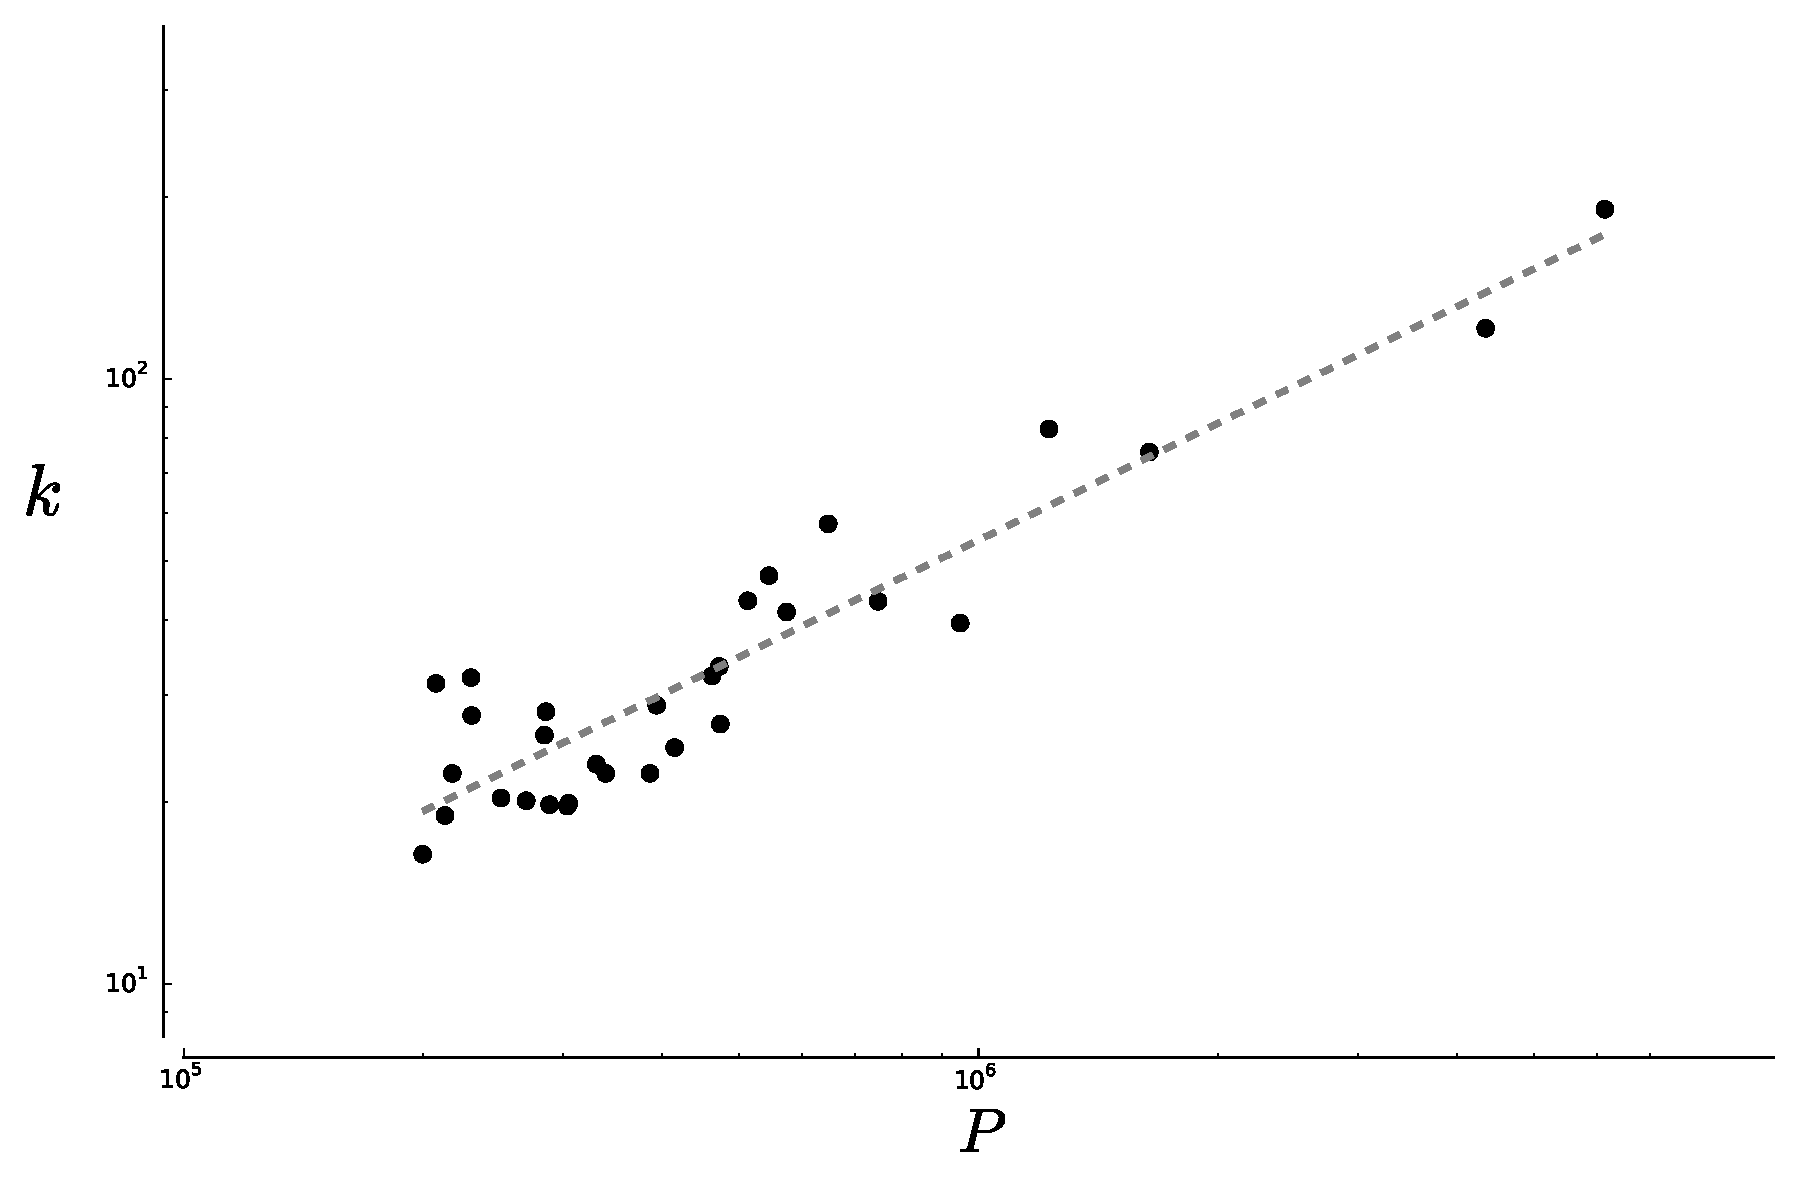
\includegraphics[width=\textwidth]{gfx/chapter-monocentric/spain_num-centers.pdf}
    \caption{{\bf Centers in Spanish cities.} Scaling of the number of centers with population for Spanish
        metropolitan areas. Assuming a powerlaw relationship, the authors
    of~\cite{Louail:2014} find an exponent $\beta = 0.64$ ($r^2=0.93$). The data
were kindly provided by Thomas Louail.\label{fig:centers_spain}}
\end{figure}

Using mobile phone data and the LouBar method to determine the number of
centers, Louail et al.~\cite{Louail:2014} also computed the number of centers
versus population for Spanish cities. 

\begin{equation}
    k_{\,Spain} \sim P^{\,0.64}
\end{equation}

Strikingly, the exponent they found is very close (equal) to the one we found on a
different system of city, using a different method to count centers, and a
radically different data collection method.\\

Taken together, the previous empirical analyses teach us that
\begin{itemize}
    \item The larger cities are, the
more polycentric they tend to be; 
    \item The average behaviour is well-approximated
by a power-law relationship between the number of centers and population;
    \item The increase of the number of centers with population is \emph{sublinear}.  
\end{itemize}

These facts calls for a theoretical explanation. We will present a model to that
effect in the next chapter. But before concluding, let us review quickly the
reasons that are traditionally invoked for the polycentric transition.

\subsection{Reasons invoked for the polycentric transition}
\label{sec:reasons_invoked_for_the_polycentric_transition}

There are numerous examples where polycentrism finds its origin in the fusion of
two Metropolises, or the incorporation of satellite
municipalities~\cite{LeNechet:2015}. The Twin Cities in the U.S., for instance:
the cities of Minneapolis and St. Paul have grown to such an extent that they now
form a single metropolitan area. The region of the Ruhr in Germany, or the
region of Tokyo in Japan are other examples. However, in this thesis, we are only interested in
an endogeneous polycentrism, caused by the growth of a single city.\\

Already in $1972$, Mills~\cite{Mills:1972} suggests that congestion might be the
cause of decentralisation and suburbanisation in large metropolitan areas.
However, we have to wait until $2003$ for McMillen to propose a thorough
empirical investigation~\cite{McMillen:2003}. The author finds a positive
correlation between the number of centers, population, and commuting cost.
Commuting cost is estimated using the peak travel time index index which is
defined as the ratio between the average travel time at peak congestion time
over the average travel time at any other time of the day. Effectively, the
commuting cost is thus a measure of the level of congestion in the city. 

In other words, the conclusion of McMillen's study is that congestion might be
the key factor to understand the polycentric transition of cities.



\section{Summary}
\label{sec:summary}

In this chapter, we have presented a historical perspective on the monocentric
hypothesis, trying to show why it appeared, disappeared, and how it is still hiding in 
some of the empirical literature. We then discussed the polycentric hypothesis,
how it was introduced, and the different methods that have been proposed to
identify and count the subcenters.

We then showed on U.S. and Spanish data that the average number of activity
centers increases sublinearly with population size. This proves, we believe, the
existence of a polycentric transition of urban areas as their population
increases. A transition, we saw, that might be due to increased levels of
congestion in larger cities. In the next chapter, we will present a model to
understand this polycentric transition. 
